\chapter{Results}
A comparison with existing game engines is difficult. ATLOD is 
developed specifically and exclusively for terrain rendering, whilst game engines
contain other components and often perform various tasks in the background, which hinders an accurate performance comparison.

\section{Experimental Setup}
\subsection{Computer}
The computer used is a MacBook Air 2020 with an Intel CPU.
The specifications are displayed in table \ref{tbl:specs}:

\begin{table}[H]
  \begin{center}
    \begin{tabular}{ c|c }
      CPU & 1.1 GHz Dual-Core Intel Core i3\\
      \hline
      Memory & 8 GB 3733 MHz LPDDR4X\\
      \hline
      Graphics & Intel Iris Plus Graphics 1536 MB\\
      \hline
      OS & macOS Monterey Version 12.6
    \end{tabular}
  \end{center}
  \caption{The specifications of the used MacBook Air 2020.}\label{tbl:specs}
  \end{table}

\subsection{Height Data and GeoMipMapping Configuration}
The height data used is the SRTM 30m data set retrieved from OpenTopography TODO cite and covers 
a large extent of Switzerland (excluding the Grisons) and small parts 
of Germany, France and Italy. The total area is 130 km$^2$.
The heightmap file
is a $13922 \times 14140$ 16-bit greyscale PNG image converted 
from a GeoTIFF file, as shown in figure \ref{fig:results-heightmap}.

\begin{figure}[H]
  \centering
  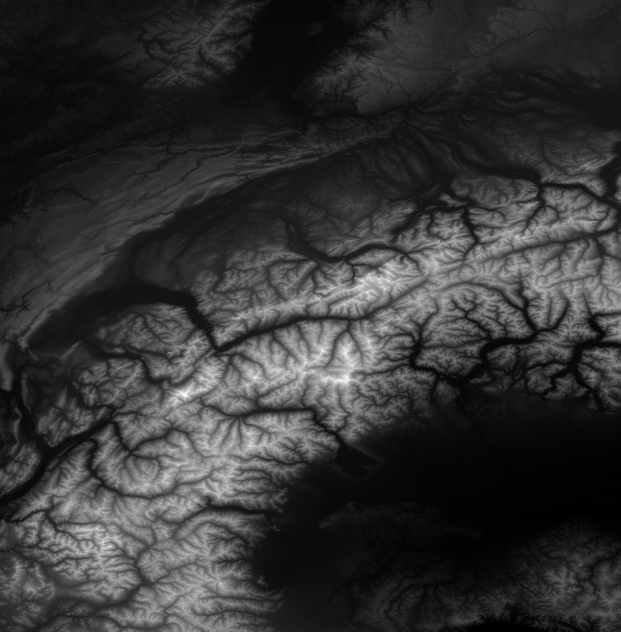
\includegraphics[width=0.7\textwidth]{results-heightmap}
  \caption{The $13922 \times 14140$ 16-bit greyscale heightmap used for benchmarking (retrieved from OpenTopography TODO cite). In this figure, the gray values were converted from 0,\dots,65535 to 0,\dots,255 in order to make the heights more visible.}\label{fig:results-heightmap}
\end{figure}

The GeoMipMapping algorithm is configured for the best balance between 
performance and visual accuracy as follows:
\begin{itemize}
  \item Block size: 257
  \item Fog: 0.003
  \item Minimum LOD: 0
  \item Maximum LOD: 8
  \item Base distance: 700
  \item LOD determination mode: Exponentially growing distance
\end{itemize}

\subsection{Benchmarks}
Two kinds of benchmarks are performed:
\begin{itemize}
  \item The first benchmark measures the performance, which measures the average FPS during rendering.
  \item The second benchmark measures the visual accuracy, i.e. the image difference between the ground truth (actual full-resolution terrain)
        and the terrain rendered with LOD.
\end{itemize}
For each of the benchmarks, two kinds of scenarios are performed:
\begin{itemize}
  \item The first scenario is the flyover from the bottom-left corner to the top-right, whilst the camera is looking down a certain angle.
        The $y$-coordinate and the front vector of the camera are fixed during this flyover.
  \item The second scenario is the $360^{\circ}$ rotation while stationary. 
\end{itemize}

\section{Performance}
\subsection{Flyover from Corner to Corner}
\subsection{360\textdegree~Rotation}

\section{Acurracy}
\subsection{Flyover from Corner to Corner}
\subsection{360\textdegree~Rotation}

\section{Theoretical Memory Consumption}
\subsection{RAM}


\subsection{GPU Memory}
While there is some complexity overhead in managing the index buffer 
in the presented way, the GPU memory usage is quite low.
The main bottleneck of this implementation in terms of GPU memory is 
the heightmap texture, which takes up 2 bytes per height value.
A solution would be to support 1-byte grayscale heightmaps. However, this would 
limit the number of possible height values to 256 and therefore produce
``blocky'' looking terrain.

On the other hand, memory consumption by the vertices and indices is quite low.
The number of vertices that are loaded on the GPU is only $b \times b$.

Table TODO shows memory usage by the heightmap texture, the vertex buffer and the index buffer 
with certain terrain sizes and block sizes.

% For example, for a block size of $2^8 + 1= 257$, the total number of vertices on the GPU is given by $257 \times 257 = 66049$, and the number of indices (manually calculated at load time) is 255086. 
% Assuming 4-byte floats for the $(x,z)$-vertices and 4-byte unsigned integers for the indices,
% the total memory taken up by the vertex and index buffer would be $66049 \times 2 \times 4 + 255086 \times 4 = 1548736 \text{ bytes}$, or 1.54 megabytes.
